\documentclass[tikz,border=2pt]{standalone}
\usepackage{amsmath}
\usepackage{amssymb}
\usepackage{xcolor}

\definecolor{journalink}{HTML}{1F1C18}
\definecolor{journalmuted}{HTML}{8A7F72}
\definecolor{journalaccent}{HTML}{9C2D2D}

\begin{document}
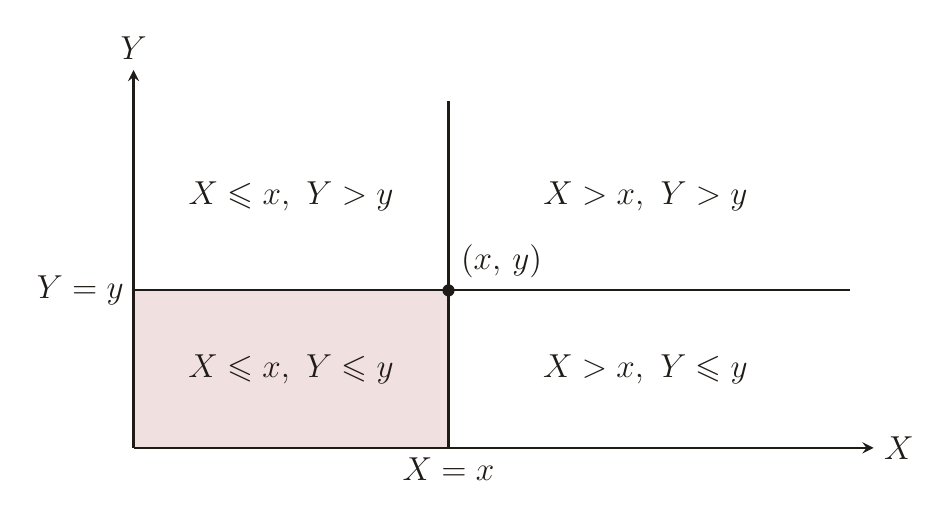
\begin{tikzpicture}[x=1cm, y=1cm, >=stealth,
                    every node/.style={journalink, font=\large}]

  %% 左下角的區域即聯合 cdf 所取的機率
  \fill[journalaccent, fill opacity=0.15] (1,1) rectangle (5,3);

  %% 兩條分界線
  \draw[journalink, line width=0.8pt] (5,1) -- (5,5.4);
  \draw[journalink, line width=0.8pt] (1,3) -- (10.1,3);

  %% 座標軸
  \draw[journalink, line width=0.8pt, ->] (1,1) -- (10.4,1) node[right] {$X$};
  \draw[journalink, line width=0.8pt, ->] (1,1) -- (1,5.8) node[above] {$Y$};

  %% 分界線的刻度標示
  \draw[journalink] (5,1) node[below] {$X=x$};
  \draw[journalink] (1,3) node[left] {$Y=y$};

  %% 四個區域
  \node at (3,2)   {$X\leqslant x,\ Y\leqslant y$};
  \node at (7.5,2) {$X>x,\ Y\leqslant y$};
  \node at (3,4.2) {$X\leqslant x,\ Y>y$};
  \node at (7.5,4.2) {$X>x,\ Y>y$};

  %% 分界點
  \fill[journalink] (5,3) circle (2.2pt);
  \node[journalink, above right, xshift=1pt, yshift=1pt] at (5,3) {$(x,\,y)$};

\end{tikzpicture}
\end{document}
